\chapter{Realizacja}
\label{cha:realizacja}
~W tym rozdziale przedstawiono sposób realizacji systemu do kontroli dostępu wykorzystującego obraz tęczówki oka jako elementu na podstawie, którego następuje rozpoznanie. System składa się ze stanowiska do akwizycji obrazu tęczówki oka oraz aplikacji generującej kod tęczówki oraz porównującej kody ze sobą. Aplikacja składa się ~z kliku modułów: wykrycie źrenicy, wykrycie granic tęczówki, tworzenie kodu tęczówki oraz ewentualnie porównania wygenerowane kodu ~z już istniejącym.

\section{Stanowisko}
\label{sec:stanowisko}
Tworząc stanowisko do akwizycji obrazu tęczówki oka należy przezwyciężyć wiele problemów. Na początek należy wybrać odpowiednią kamerę ~i obiektyw. Wybór kamery był ograniczony zasobów laboratorium, ~w którym było tworzone stanowisko. Do realizacji wybrano kamerę !!!!TU WSTAWIĆ NAZWĘ!!!!.

Do wybranej kamery należało dobrać obiektyw. Ponieważ naszym celem było otrzymanie ostrego obrazu ~w dużym powiększeniu odległości oraz dużej głębi ostrości należało wybrać obiektyw o możliwie dużej ogniskowej. Zdecydowano się wykorzystać najlepszy dostępny obiektyw !!!!!TU WSTAWIĆ NAZWĘ!!!!.

Kolejnym problemem, który należało pokonać były odblaski na powierzchni oka. Odblaski takie powstają ~w wyniku odbicia się światła pochodzącego od światła zewnętrznego oraz od światła żarówek ~i jarzeniówek świecących ~w pomieszczeniu. Głównym problemem były odblaski powstające na tęczówce oraz źrenicy, ponieważ te elementy obrazu poddawane są analizie. Najprostszym sposobem pozbycia się takich odblasków jest zasłonięcie drogi promieni świetlnych od źródła do oka. Zrealizowano to za pomocą kartonowego pudła szczelnie, ~w którym umieściliśmy kamerę. Osoba badana umieszcza głowę na granicy pudła, co pozwala na uniknięcie odblasków. Dodatkowo głowa badanej osoby jest umieszczona na stojaku, którego zadaniem jest unieruchomienie głowy, dzięki czemu uchwycony obraz ma lepszą ostrość (nie jest ,,ruszony'').

Wadą zastosowania kartonowego pudła jest zmniejszenie jasności uzyskiwanych obrazów. Do rozjaśnienia obrazu użyto oświetlacza IR oraz lampy umieszczonej na kamerze, która oświetla oko badanej osoby. Taka lampa również tworzy odblask, lecz ~w tym wypadku odblask może być wykorzystany przez algorytm wykrywający źrenicę. Jest to możliwe, ponieważ ~z uwagi na umiejscowienie lampy odblask powstaje na środku źrenicy, dzięki czemu jest łatwo znaleźć ten środek. Obraz jest zapisywany ~w skali szarości.

Ponieważ obrazy osiągnięte ~z użyciem pierwszej dostępnej kamery nie były zadowalające należało użyć innej kamery. Głównym problemem była mała rozdzielczość kamery oraz mała jasność ~w pudle. Przy użyciu kamery !!!Nazwa!! te problemy zostały zniwelowane. Kamera ma ~o wiele większą rozdzielczość. Ponadto problem zbyt małej jasności został zniwelowany tylko ~z użyciem oświetlacza IR. Nie było potrzeby użycia innej lampy, co ułatwiło dalsze przetwarzanie zarejestrowanych obrazów.


\section{Wykrycie źrenicy}
\label{sec:wykrycieZrenicy}
Część algorytmu odpowiedzialna za wykrycie źrenicy ma za zadanie odnalezienie źrenicy na obrazie oraz opisanie kształtu źrenicy jako okrąg. Zadanie to jest realizowane ~z wykorzystaniem wcześniej wspomnianego odblasku pochodzącego od lampy, który powinien znajdować się na środku źrenicy. Odblask jest jednym ~z najjaśniejszych punktów na obrazie. ~w związku ~z tym wykrycie odblasku odbywa się ~z wykorzystaniem binaryzacji ~z progiem 254. Po tej operacji na obrazie zostają tylko piksele najjaśniejsze (jak na rysunku \ref{fig:binaryzacja}). Niestety na wielu ujęciach odblask na źrenicy nie jest jedynym, który jest widoczny na obrazie. Pozostałe mogą znajdować się ~w różnych miejscach: na białku oka lub na skórze. Można ten fakt wykorzystać analizując otoczenie znalezionych odblasków. 
\begin{figure}
\begin{center}
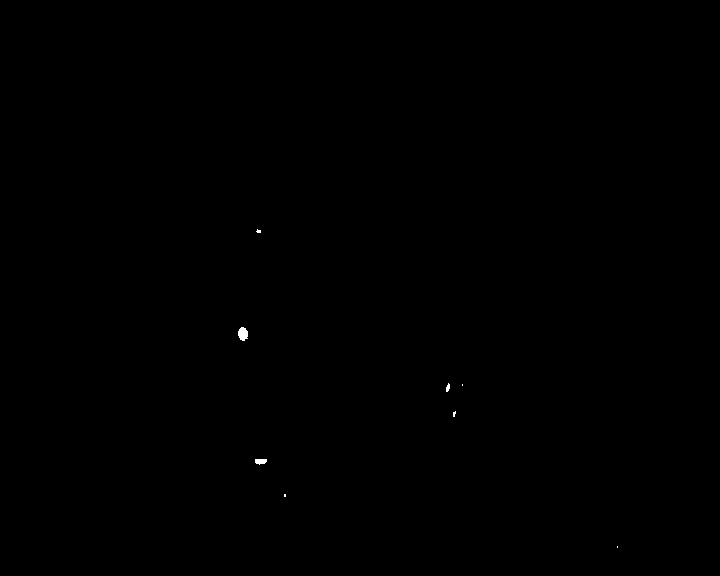
\includegraphics[scale=0.5]{binaryzacja.jpg}
\caption{Obraz po binaryzacji, jasne punktu to znalezione odblaski}
\label{fig:binaryzacja}
\end{center}
\end{figure}

Interesujący nas odblask znajduje się ~w otoczeniu źrenicy, ~a więc jednego ~z najciemniejszych obszarów obrazu, otoczenie pozostałych odblasków jest o wiele jaśniejsze (skóra lub białko oka). Dlatego algorytm analizuje otoczenie każdego odblasku. Badanych jest 20 pikseli ~w odległości od 10 do 20 pikseli. Wybierany pierwszy odblask, ~w którego otoczeniu większość pikseli ma jasność poniżej 50. Po znalezieniu jednego piksela odblasku łatwo można znaleźć cały odblask. Jest to realizowane przez analizę otoczenia znalezionego piksela (~w odległości nie większej niż 25 pikseli) ~i klasyfikowaniu ich jako element odblasku jeśli ich jasność jest większa niż 240. Przykład wyniku przeprowadzonych operacji jet przedstawiony na rysunku \ref{fig:dobryOdblask}.
\begin{figure}
\begin{center}
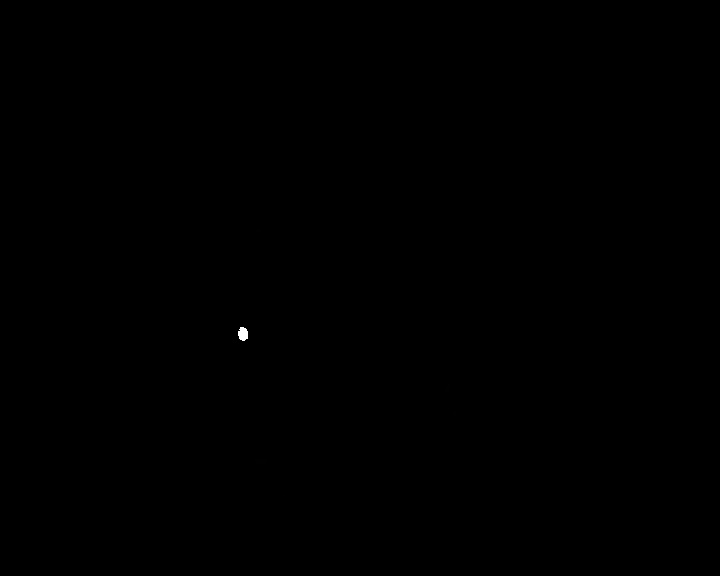
\includegraphics[scale=0.5]{odblask.jpg}
\caption{Obraz po realizacji algorytmu poszukiwania odblasku na źrenicy}
\label{fig:dobryOdblask}
\end{center}
\end{figure}

Po znalezieniu wszystkich pikseli należących do odblasku jego kształt jest aproksymowany kołem, którego środek jest przyjmowany jako środek źrenicy. Mając środek źrenicy można zastosować metodę ,,eksplodujących okręgów'' ~z patentu Daugmana. Szukane jest największe zmniejszenie się jasności pikseli na rozszerzającym się okręgu (~z uwagi na to, że źrenica jest ciemna ~a tęczówka jest jaśniejsza). Znaleziony okrąg określa źrenicę. Przykład obrazu z wykrytą źrenicą jest przedstawiony na rysunku \ref{fig:zrenicaNasza}.
\begin{figure}
\begin{center}
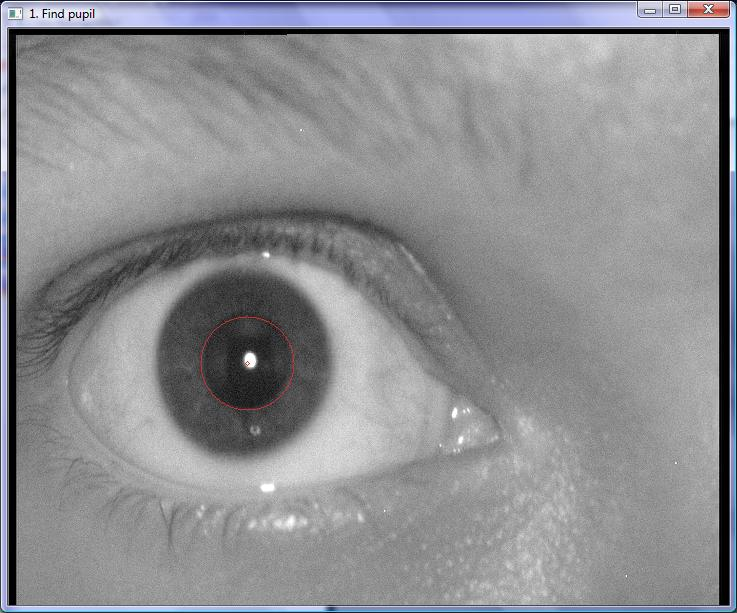
\includegraphics[scale=0.5]{zrenica.jpg}
\caption{Wykryta źrenica}
\label{fig:zrenicaNasza}
\end{center}
\end{figure}

\section{Wykrycie tęczówki}
\label{sec:wykrycieTeczowki}
Algorytm odpowiedzialny za wykrycie tęczówki jest identyczny jak ~w pracy \cite{Gl11}. Przykładowy obraz z wykrytą tęczówką jest przedstawiony na ryskunku \ref{fig:teczowkaNasza}.
\begin{figure}
\begin{center}
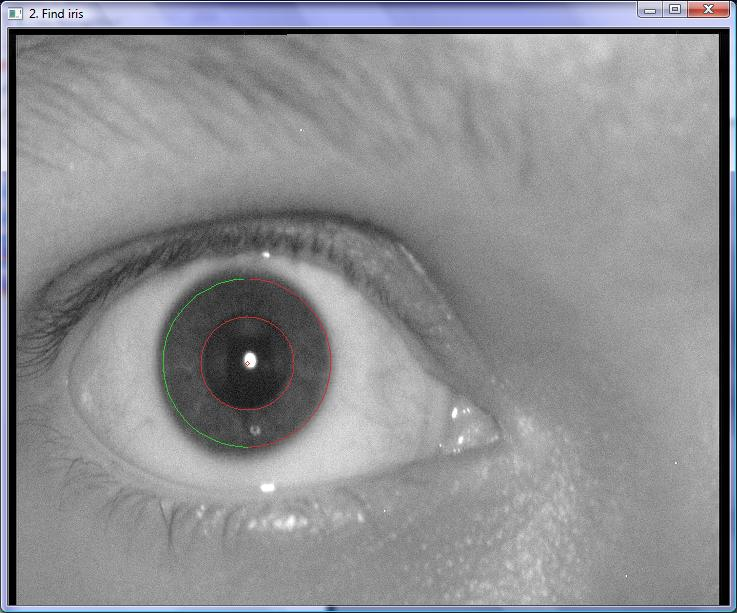
\includegraphics[scale=0.5]{teczowka.jpg}
\caption{Obraz po realizacji algorytmu poszukiwania granic tęczówki}
\label{fig:teczowkaNasza}
\end{center}
\end{figure}

\section{Ekstrakcja cech tęczówki}
\label{sec:ekstrakcja}
Zadaniem części algorytmu odpowiedzialnej za ektrakcje cech tęczówki jest zmniejszenie ilości danych reprezentujących daną tęczówkę. Po tej operacji zostaje utworzony wektor o długości 2048 bitów. Dzięki temu można znacznie ograniczyć liczbę przechowywanych danych, potrzebnych do poprawnego rozpoznania osoby. Ważne jest, by otrzymany wektor był wyraźnie różniący się pomiędzy różnymi osobami oraz dla jednej osoby różne zdjęcia generowały podobny zestaw bitów. 

~w celu określenia cech danej tęczówki stosuje się filtry Gabora określone wzorem (tu będą wzory ale na linuxie to zrobię)

Obraz jest filtrowany ~z użyciem otrzymanych filtrów. Po tym zabiegu otrzymujemy współczynniki zespolone, które sumujemy ~w pewnych obszarach. Obszary wybierane są na tęczówce ~w punktach zależnych od jej rozmiaru. Jest to spowodowane tym, że ~w zależności od jasności otoczenia źrenica się zwiększa lub zmniejsza co powoduje zmniejszanie lub zwiększanie tęczówki. Otrzymana suma kodowana jest ~w ten sposób, że osobno rozpatrując część rzeczywistą ~i urojoną zapisywane jest 1 ~w przypadku, gdy suma jest większa od zera oraz 0 jeśli jest mniejsza lub równa. ~w ten sposób otrzymujemy 2 bity na jeden obszar. Ponieważ stosujemy 8 różnych orientacji filtru Gabora to potrzebujemy 2048/(2*8) = 128 obszarów. Obszary wybierane są po dwóch stronach tęczówki, więc potrzeba po 64 obszary na jedną stronę. Przykład wyznaczonych obszarów przeznaczony jest na rysunku \ref{fig:obszaryNasze}.
\begin{figure}
\begin{center}
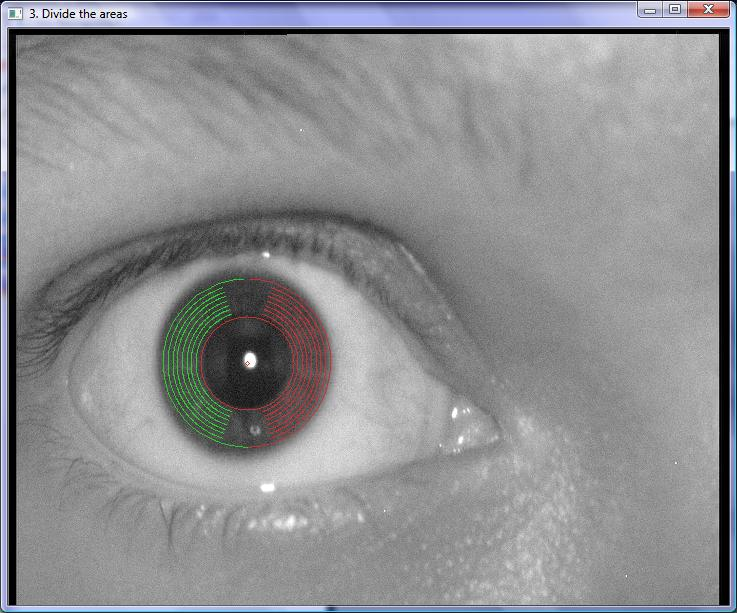
\includegraphics[scale=0.5]{obszary.jpg}
\caption{Obraz z zaznaczonymi obszarami używanymi do tworzenie kodu tęczówki}
\label{fig:obszaryNasze}
\end{center}
\end{figure}

\section{Porównanie kodów tęczówki}
\label{sec:porownanieKodow}
~W celu określenia czy dane dwie tęczówki należy do jednej osoby należy porównać otrzymane kody. Porównanie wykonywane jest za pomocą operacji XOR zgodnie ze wzorem \ref{eq:Hamming}.
\begin{equation}
\label{eq:Hamming}
H = \sum \frac{XOR(A,B)}{2048}
\end{equation}
gdzie:
$A, B$ - porównywane kody tęczówek, każdy o długości 2048 bitów.\\
Po tej operacji wartość $H$ określa procent różnych pikseli dla dwóch różnych kodów.

Osoba może mieć trochę obróconą głowę ~w czasie robienia zdjęcia służącego identyfikacji ~w stosunku do zdjęcia, ~z którego powstał zapisany kodu ~w bazie. ~W celu zminimalizowania błędu stosowana jest rotacja jednego z porównywanych kodów. Kod jest przesuwany ~w obydwie strony ~o dwa piksele (ponieważ ~z jednej lokalizacji na obrazie otrzymujemy dwa bity kodu). Wykonywanych jest 9 porównań kodów. Wybierana jest najniższa wyliczona wartość odległości Hamminga. Ustalonym progiem zgodności dwóch kodów jest 0.32 \cite{Daugman}.
